\section{Beginning the project}

As a new Javascript developer, the first few weeks of coding was spent learning the language and becoming familiar with how it all worked. This included knitting Javascript together with HTML and CSS. By using this combination of programming languages, Requirements \ref{ssection:hard1} and \ref{ssection:hard2} will be automatically met and this was the reason why these languages were chosen in Section \ref{section:proglang}.

For any software project, keeping a good record of progress is important. In this case, GitHub was chosen as the version control. GitHub was simple to set up and use. As well as it being used to  maintain an archive of the project I also used to to store notes as the project progressed. If a bug has been introduced in the version under development it is straightforward to revert to a previous committed version and carry on again from then. This project is stored in a public repository meaning that anyone can view the code if they want to. This makes the code open source and anyone can download and edit the code is they choose. This supports Requirement \ref{ssection:nfun5} and hopefully interested parties will contribute to the project and take it further.

Learning how to use the HTML 5 canvas as well as the methods associated with this that were available took some getting used to. I started off by creating a small game that was played on a HTML canvas. The user would use a button to create numbers. They could drag and drop these numbers on top of each other. If they dragged an item over the top half of another item then the two numbers would subtract from each other and if over the bottom, then the two numbers would add.

\begin{figure}[H]
\centering
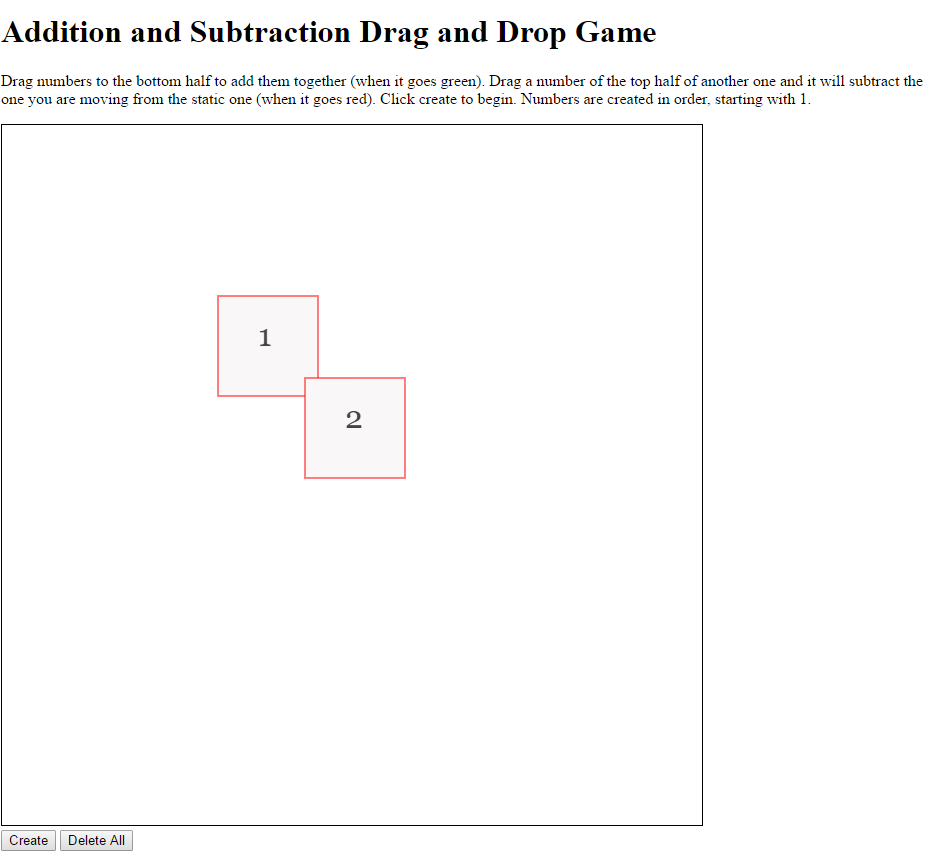
\includegraphics[scale=0.4]{addition1}
\caption{The first game I created with Drag and Drop}
  \label{fig:addition1}
\end{figure}

This game helped to understand how drag and drop worked, as well as understanding how items can react differently on a screen depending where the mouse is released. Most of this code is carried forward and used in the main Natural Deduction game.

\section{Drag and Drop}

With no prior experience of implementing a drag and drop system, an online tutorial was followed and ideas were expanded from these foundations. \cite{Howt28:online} This was the tutorial that was used for both the initial addition game and also for the main software project.

The three functions created in drag and drop are all event based. These events trigger when the left mouse button is clicked down, when the mouse is moved and when the mouse is released. All three functions have important roles and do different jobs that make the drag and drop successful. These functions were implemented according to the way it was described in the design.

\begin{figure}[H]
\begin{lstlisting}[language=JavaScript]
function myDown(e){ //When the mouse is pressed down
	move = 0;
	for (j = 0; j < r.length; j++) { //Discovers which item is pressed down.
		if (e.pageX < r[j].x + (r[j].w/2) + canvas.offsetLeft && e.pageX > r[j].x - (r[j].w/2) +
			canvas.offsetLeft && e.pageY < r[j].y + (r[j].h/2) + canvas.offsetTop &&
			e.pageY > r[j].y - (r[j].h/2) + canvas.offsetTop){
				move = j;
				r[j].x = e.pageX - canvas.offsetLeft;
				r[j].y = e.pageY - canvas.offsetTop;
				dragok = true;
				canvas.onmousemove = myMove;
				break;
		}
	}
}
\end{lstlisting}
\caption{The function executed when the left mouse button gets pressed down}
\label{fig:myDown}
\end{figure}

When the left mouse button is pressed down, an event handler runs, which runs the function runs the function in Figure \ref{fig:myDown}. The function iterates through all of the objects on screen. These objects are stored in the array 'r' and this function sees if the location of the mouse click is in the same position as any of the objects. If this is the case then the variable 'dragok' is set which indicates that an element needs to be moved. 

The moving mouse function 'myMove' is constantly executed on mouse movement, but the majority of logic within it is only run when an object on the screen is selected to drag and drop because 'dragok' is set to true. The logic within the moving function went through different phases of development as the project progressed. Explained in detail below is both the legacy system and the new, improved way that it now works.

\subsection{Original Colour System}

This first drag and drop algorithm implemented was simpler and based on the design in Figure \ref{fig:Design3}. This worked effectively and was based on the positioning of all of the objects on the screen. Thought had to be given to how the system would react when items were dragged on top of each other. The initial thinking was to base what happened to objects on the location of other objects. 

The tree structure of natural deduction proofs means that the visual representation naturally splits into four different parts. Top left, bottom left, top right and bottom right are all possible locations where a part of a proof can be located. The original system worked out the location of all the objects on the screen. If another object was dragged over one of the objects, then depending which corner it was dragged over, the algorithm will set the borders of the two objects of a certain colour. Different colours would be set depending on what type of object is being highlighted. 

Variables and conditionals can be dragged onto other objects of the same type. In Figure \ref{fig:Conjunction} below, dragging the conjunction onto the right hand side of the 'A' outlines both objects in red. Dragging the conjunction to the left hand side of the 'A' sets both of the borders green.
 
\begin{figure}[H]
\centering
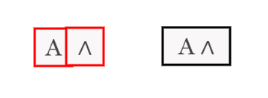
\includegraphics[scale=0.75]{AConjunction}
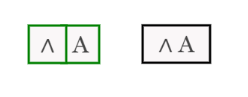
\includegraphics[scale=0.75]{ConjunctionA}
\caption{How to join statements together}
 \label{fig:Conjunction}
\end{figure}

The same logic applies to proof structures as shown in Figure \ref{fig:oldColour} below, but all four of the corners could be dragged over to give different coloured borders. Releasing the mouse button when the borders are highlighted removes the object that is being dragged and places whatever is on the moving object to the static element in the correct corner.  

\begin{figure}[H]
\centering
\centerline{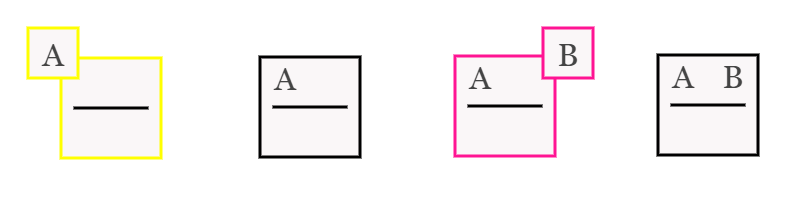
\includegraphics[scale=0.7]{oldColour}}
\caption{How combining statements to proofs worked in the original version}
 \label{fig:oldColour}
\end{figure}

The advantage of this method is that it makes it clear which part of the proof the user is dragging to. The use of colours makes it clearer to the user and it means once a user is familiar with it, they will learn what to do in future. This may be considered a disadvantage because it does not come across as intuitive because the colours are unknown to the user before they start the game. There are also no obvious points on the proof where the user can drag to, and without any kind of prompt it can be difficult about the possible valid moves available.

Another issue occurs when multiple layers of proof are dragged together. This system of associating colours with the area user drags the objects to does not work intuitively when building proofs. Natural deduction proofs are often built from the bottom up. With this method, proofs cannot be built from bottom up because the dragging and dropping is all associated with the first object that is dragged onto. Any new proof dragged onto the top left or top right of the proof will remove the existing structure that is there. This leads to a peculiar way of forming proofs of multiple layers. Due to these reasons and reacting to feedback echoing this, the way users dragged onto objects was changed.  

\subsection{The Dots System} \label{ssec:dots}

A redesign of the drag and drop algorithm made the software fulfil Requirement \ref{ssection:fun1} more effectively, so it was a positive step, even if it was more technically challenging. The idea behind this was to indicate to the user what moves were valid. The goal of the new system was also to provide a more flexible way of creating proofs, where users could drag onto any part of proof that was missing. This was achieved by adding dots to the proof structure.

Dots are used to indicate to the user where they can drag onto on the proof. It makes it much clearer visually and it is more intuitive. Locations of each dot needed to be stored. This meant that every dot had to be a separate object with its own unique ID number and location information. These ID numbers would link to every proof object, so each proof object that can be dragged and dropped knows which dots are associated with it.

Also in the dot object is the colour of the border. If one of the objects is dragged over the location of the dot, then both the dot and the object being dragged over will turn purple. This is to let the user know which elements are being highlighted and what is going to happen if the user releases the mouse. This is a great improvement on the previous system and will reduce errors from the user because it is less likely that the user will make mistakes.  

\begin{figure}[H]
\centering
\centerline{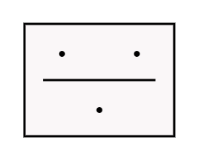
\includegraphics[scale=0.5]{dots}}
\caption{The new representation of the ``2 Top/1 Bottom" proof structure}
 \label{fig:dots}
\end{figure}

Another improvement from the first iteration of the code is that this system is more natural in the way proofs are created. Proof structures can be dragged onto the dots at the top of the current structure which leads to building a proof from bottom up. This is the conventional way to create Natural Deduction proofs in the tree structure and will offer a more realistic experience to the user.

In this way of dragging and dropping, the border of the object does not change colour when the user drags onto it. Only the dot of the static object changes colour. Dragging to any corner of the object no longer has any effect, it is all based on where the dots are located. Because of this, multiple layers of proof can be built up with lots of dots contained in them. The user can then individually drop variables or statements onto the dots. This was something that was not possible in the previous way of dragging and dropping.

\begin{figure}[H]
\centering
\centerline{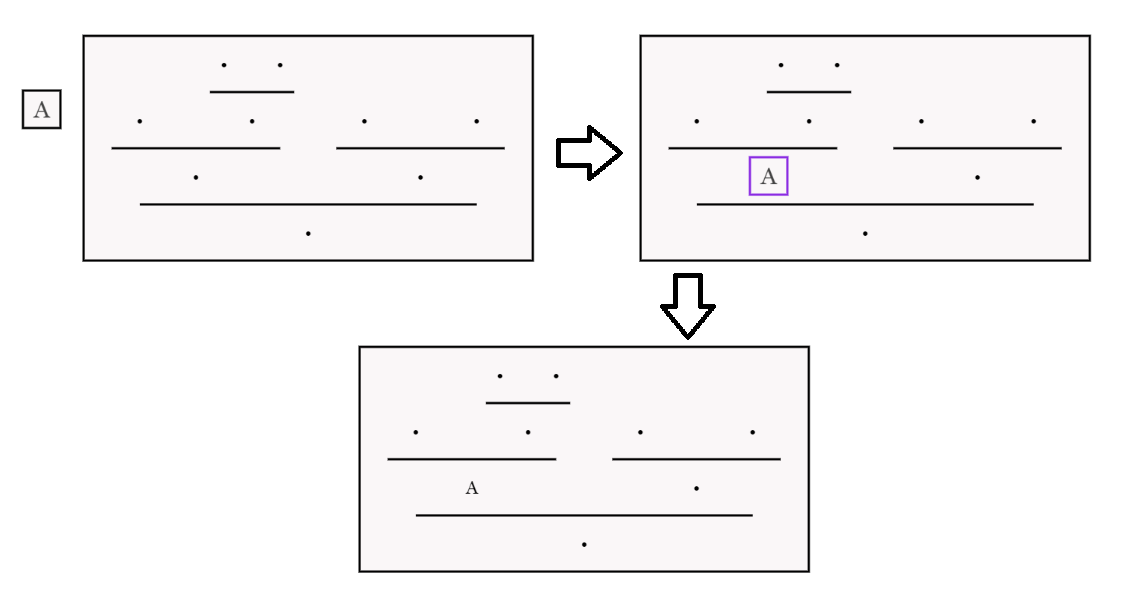
\includegraphics[scale=0.5]{dotsdnd}}
\caption{Example of how a user can drag onto a dot}
 \label{fig:dotsdnd}
\end{figure}

When another structure is placed on top of a dot, the dot object is replaced with the structure that the moving object has, whether that is another proof structure or a statement. This method of dragging and dropping proofs solved both of the main issues encountered in the original colour system. This is based on continuous development and unit testing as well as constant dialogue with interested stakeholders such as the project supervisor Willem. Constant testing and improvement is a key part of any software project and will be covered in further detail later.  

\section{Data Structures}

Due to the visual representation of the proofs as trees, storing the data in a similar way made sense as it made the design scalable. Basic objects are stored as a list. Each draggable object structure was the same, whether it was a proof structure or a variable. The core structure had four elements. The first element represented the top left corner, the second element represented the top right corner and the third and forth elements represented the bottom left and right corners respectively.

If an object is just a statement, like a variable, connector or a mixture of these, the string representing the statement would be placed in the first element and the remaining three elements would contain ``\%". A percentage string was one that let the program know that this element will never need to be used for this part of the proof. For the statement A $\wedge$  B, the data structure would be represented as [``A $\wedge$  B", ``\%", ``\%", ``\%"].

These percentage strings were also used for determining the layout of a tree structure. Two elements on the top and one on the bottom is used as well as one element on the top and one on the bottom in this game and they are represented with the following data structures:

\begin{figure}[H]
\begin{center}
\begin{tabular}{ |c|c|c| } 
\hline
2 Top / 1 Bottom &  [``A", ``B", ``A $\wedge$ B", ``\%"] & \raisebox{-.5\height}{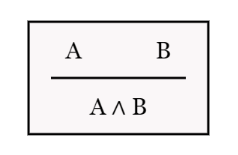
\includegraphics[scale=0.5]{2Top1Bottom}} \\
\hline
1 Top / 1 Bottom &  [``A $\wedge$ B", ``\%", `` B", ``\%"] & \raisebox{-.5\height}{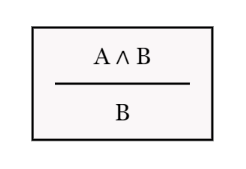
\includegraphics[scale=0.5]{1Top1Bottom}} \\
\hline
\end{tabular}
\end{center}
\caption{Simple data structures}
\label{tbl:table1}
\end{figure}

When dots are represented in the proof, the ID number of the dot number is the element in the proof structure. The drawing algorithm will recognise a number and render it in a dot. The ID numbers of the dot will link to a dot and the dot object with the position coordinates associated with it.

The way larger proof trees are stored is in the form of nested lists. If an element of the list is stored as another list, then a proof structure of the same format can be contained there. This system works recursively to create proofs in tree shapes, which can then be easily be drawn by the software.

Proofs with dots and multiple layered proofs are represented as follows:

\begin{figure}[H]
\begin{center}
\begin{tabular}{ |c|p{4.5cm}|c| } 
\hline
Dots in a proof &  [1, 2, 3, ``\%"] & \raisebox{-.5\height}{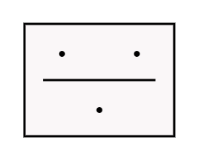
\includegraphics[scale=0.5]{dots}} \\
\hline
Multi-line Proof &  [[``A", ``B", ``A $\wedge$ B", ``\%"], ``C", ``(A  $\wedge$ B) $\wedge$ C"] & \raisebox{-.5\height}{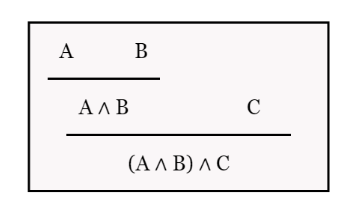
\includegraphics[scale=0.5]{multiline}} \\
\hline
\end{tabular}
\end{center}
\caption{Additional data structures}
\label{tbl:table2}
\end{figure}

A simple, unified proof system allows both ease when drawing and when assessing the proof to check whether it is valid. As the structure is consistant, comparison is possible.

%\section{Unification Algorithm}

%An important requirement for this software project was to recognise whether a proof is valid and correct. In Natural Deduction logic you can't use distributive, associative or communicative %properties. \cite{intro} Every proof needs to be shown explicitly. This means that Natural Deduction proofs can only be reordered where the substance of every branch is the same, but the %location in the proof can be different.

%As the simple example shown in Figure \ref{fig:unification} consider A $\wedge$ B. Having both A and B on the top line states that A is true and B is true. Whether the A is on the left or the B i%s on the left is irrelevant but this shows that proofs can be represented differently. A whole proof tree can look very different whilst representing the same proof logically and this project %provides an algorithm that achieves this.

%\begin{figure}[H]
%\centering
%\centerline{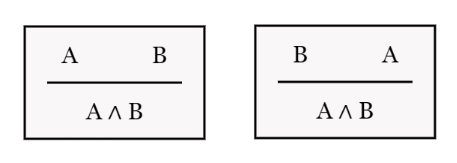
\includegraphics[scale=0.5]{unification}}
%\caption{Two valid ways to represent A$\wedge$B that will both be accepted by the Unification Algorithm}
%\label{fig:unification}
%\end{figure}

%The key part to this algorithm is that is uses recursion. The algorithm makes sure that a branch of the tree matches a branch of one, ideal solution that is provided. If this branch is correct then %other branches are checked, again by recursion. If all branches in the user's answer are accounted for and match up with the ideal answer given then the solution is valid. If any one of the %branches doesn't match up then the proof is incorrect. It will return that the user's proof is incorrect and allow the user to try again.

%By having this generic algorithm in place, it makes the system very flexible and extensible. Adding levels is incredibly easy because only one valid proof needs to be submitted and then all of %the valid solutions will be permitted. This makes the software both adaptable and easily scalable which are another two key requirements for this software. 

\section{Drawing and rendering algorithms}

The drawing algorithm is another important part of the software to make sure that the proof is presented to the user in the way that they expect. Presenting information to the user correctly and reliably is a key feature that this project must achieve. The drawing algorithm uses \textit{setInterval} which is a Javascript function that calls a function at certain intervals. The function called contains the drawing algorithm that redraws what is on the canvas, giving a user instant feedback to whatever moves they are performing.

The drawing algorithm has been written in a way that it interprets the data structure to correctly render the proof in a tree shape. The drawing algorithm takes into account whether each structure is ``2 Top/1 Bottom" or ``1 Top/1 Bottom" and draws it appropriately. It also takes into account any dots in the system, which are represented as numbers in the proof system. The algorithm recognises these numbers and renders them as a dot to the user. 

Figure \ref{fig:myDown} gives a flavour of the complexity of drawing the proof. This Figure shows whether a dot or text should be rendered in the top left of a proof structure. If neither of these things are here because the proof is ``One up/ One down" or that there is a proof structure above this point, then it will go into different logic of the algorithm.   

\begin{figure}[H]
\begin{lstlisting}[language=JavaScript]
if(text[0] != "%" && text[1] != "%" && (typeof text[0] === 'string' || typeof text[0] === 'number')) {
		//'%' in text[1] would mean one statement at the top of the proof.
		//A string means some statement can be written, a number represents a dot.
		ctx.fillStyle = "black";
		if(typeof text[0] === 'number'){ //Dot
			if (dotsArray[text[0]].formula != ""){    //If a statement has been dragged on 
				temp = dotsArray[text[0]].number;     //to an object, change the array to 
				text[0] = dotsArray[text[0]].formula; //represent that statement in the object
				if(typeof text[0] === 'string'){
					ctx.fillText(text[0], x-(w/4), y-dist);
				}else{ //Proof structure dragged on
					if (typeof text[1] === 'string' || typeof text[1] === 'number'){
						r[i].proofHeight = r[i].proofHeight + r[move].proofHeight - 1;
					}
					r[i].dots = (r[i].dots).concat(r[move].dots); //Update the dots an object holds
					r.splice(move,1); //remove the old object from the canvas
				}
				dotsArray[temp].number = "deleted"; //ignore the dots in the old object
			}
			else {
				dotsIterate(text[0], x-(w/4), y-dist); //update position of dots 
				ctx.fillText(".", x-(w/4), y-dist);
			}
		}			
\end{lstlisting}
\caption{A code snippet from the drawing algorithm}
\label{fig:myDown}
\end{figure}

The main point to understand from this code is that dots are represented by objects and the position location of them needs to be updated. The visual representation of the dot object needs to be a dot string, even though it is represented as a number in the array structure. This code gives an example of the complicated logic going into drawing canvas items correctly.

Multi level proofs need to be drawn in a different location of the screen because they are on top of the first level of structure. Due to the potentially different proof widths that need to be drawn, the first 4 levels of proof are individually accounted for. If more that four levels of proof need to be drawn, a recursive function is used. Another box linking to the proof is drawn in the same format as the original proof. This is done for ease of readability for the user and with Requirement \ref{ssection:fun3} in mind. The user will still be able to read all parts of the proof easily.

In retrospect, a better drawing function could have been implemented. One that offers the whole proof in one object, no matter how tall the proof. As long as it remains readable, it would be ideal. An algorithm that uses recursion more would reduce repetitive code. Tree like structures lend themselves well to recursion, so this could have been utilised more. 

A feature that works well is the resizing of boxes. When the height of a proof is increased, the size of the box will automatically increase as well. As the height increases, the width will also increase proportionally as well. This is to make sure that items on the top row on the proof will still be rendered clearly and that the user has a good user experience.

\section{The Game Play}

Although making sure the mathematical logic was complete and works successfully, it is just as important to provide the user with an enjoyable game in accordance with Requirement \ref{ssection:fun9}. There are many tools already available that will aid a user in learning Natural Deduction, but as previously discussed, many of these do not engage the user and lack other key elements that make these tools into games. Part of the implementation of this project was putting in key gamification attributes that would make this tool a game.

One of the main features that was important to include was the concept of levels.(Requirement \ref{ssection:fun7}) These are set up with guidance to help the user through the game. The implementation of levels in this game prevents the user from using certain elements and this helps the user by guiding them in what buttons they can press. In Figure \ref{fig:buttons} below, which represents the buttons in Level 1 of the software, only the buttons needed to create A $\wedge$ B are available to press. Buttons unavailable are greyed out and when the user hovers the mouse over the button, a 'not allowed' symbol is displayed. These buttons use bootstrap and are toggled in the Javascript by setting a property whether they should be enabled or disabled.   

\begin{figure}[H]
\centering
\centerline{
\includegraphics[scale=0.65]{buttons}}
\caption{How Buttons are represented in the game}
\label{fig:buttons}
\end{figure}

Requirement \ref{ssection:fun4} set out to let the use experiment with creating proofs. This is implemented in part by the implementation of a Freeplay button. Figure \ref{fig:buttons} displays the Freeplay button which the user can turn on and off at any time. Pressing this button makes all of the other buttons available to the user (they can be pressed) apart from the the 'Check Proof' button. The level objective is also removed. A user can still drag and drop everything but the proof cannot be compared to anything. Unfortunately the user cannot save their proof so it is currently unavailable for a user to create their own levels. This would be something I would consider in the future work as it would let the software be more scalable. 


An important requirement for this software project was to recognise whether a proof is valid and correct. In Natural Deduction logic you can't use distributive, associative or communicative properties. \cite{intro} Clicking on 'Check Proof' runs the checking algorithm. This will either complete the level and start the next one if the user is correct. If the user is wrong, it will let them try again. The pop up that appears when a user gets the proof incorrect displays the part of the proof where it is first incorrect. This helps the user and gives them a guide of which part of the proof they should look at. The implementation of this checking system gives the user hints, gives them instant feedback which are both requirements and fulfils Requirement \ref{ssection:fun5} which explicitly states the need for a checking system.

A user gets a score of 10 for every level successfully completed with no mistakes. Every mistake they make (that is when they click 'Check Proof' and the proof is incorrect) is a deduction of two points. A user successfully completing a level correctly will always receive 1 point, no matter how many attempts are taken. Scores for all the levels are accumulated and a final score for a user is given. Having a score was one of the key gaming elements set out in Requirement \ref{ssection:fun8} and this offers a competitive aspect of the game. The user can then play the game again and hopefully the user can keep trying until they get a perfect score of 10 for every level. Scoring is included to motivate the user to play again and hopefully subconsciously solidify the knowledge the user is learning about Intuitionistic Logic and the Natural Deduction Proof System.  

Additionally, further help is provided via a hints button that has been implemented. This is to aid the user in the learning process. Clicking the hints button reduces the score by 2 points, so it encourages the user not to use the hints, but they are available if needed. Having hints available to the user lets them continue with gaming process without getting frustrated. This will hopefully stop the user from giving up and they will persevere more by using the hints. (Requirement \ref{ssection:fun6})

\section{Design Implementation}

The first design principle was to make the game look aesthetically pleasing to the user. To help with this, Bootstrap was used, which is a responsive front end framework. \cite{Boots82:online} Using Bootstrap meant that whatever the size of the window, the buttons, title and the level objective were always visible to the user. Due to the drag and drop functionality of the canvas, this is a fixed size, so if it is not suitable then the user needs to resize their window or zoom in or out to successfully play the game.

All of the levels have a consistent layout, with the canvas in the same place. The buttons are always below the canvas and the level goal is always above the canvas. Having this familiarity means that the user will find the software easy to navigate. This consistent look to the software means the user will quickly pick up what they need do and then will be more comfortable as they progress through the levels.

Testing that has gone on throughout the development process means the user should feel in control of the system because there will be nothing unexpected. This resonates with the consistent design, so the user knows that what they expect to happen does happen. Figure  \ref{fig:game} shows the user interface that has been created in accordance with the design. It shows the main gaming page with the hints visible.

\begin{figure}[H]
\centering
\centerline{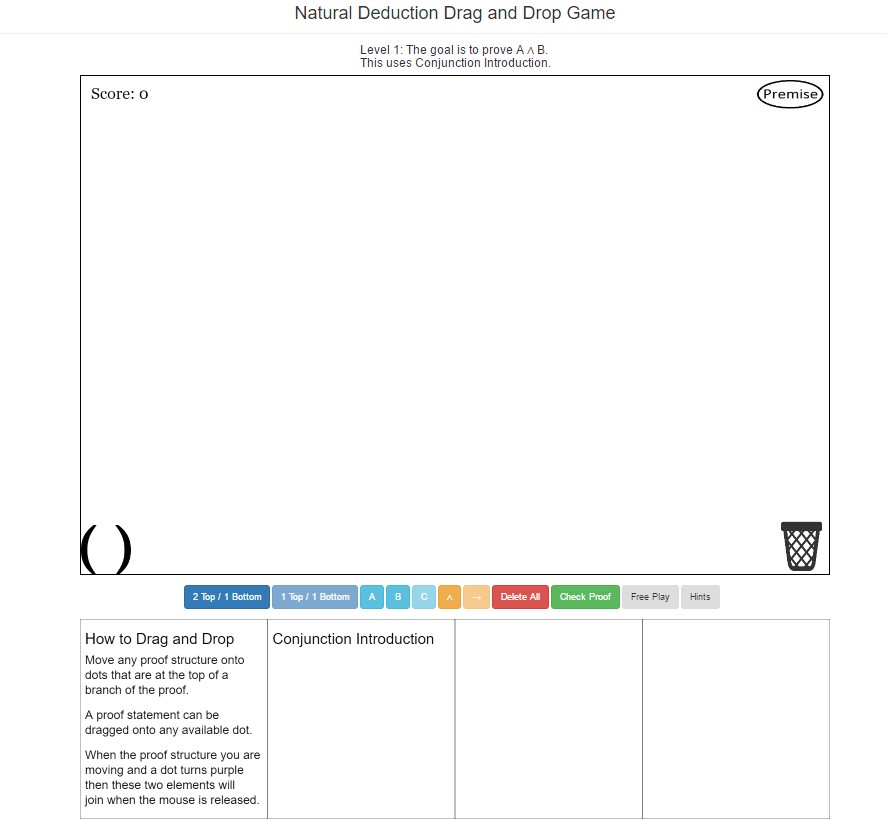
\includegraphics[scale=0.65]{game}}
\caption{The interface of the game}
\label{fig:game}
\end{figure}